\section{Additional accounting and secondary-model experiments}
\label{app:secondary}

The primary comparison in the main text uses AR-30B and DiffusionGemma.
The AR-3B results below are auxiliary experiments with a smaller dense
Qwen2.5 model; they do not establish either quality equivalence or
chain-level speedups for AR-30B. LLaDA is another diffusion baseline and
is not a substitute for DiffusionGemma in the main comparison.

\subsection{Output-budget accounting and energy}
\paragraph{Output budget is not generated length.}
Table~\ref{tab:niche} retains the original serial-sweep means so that
the fitted cost model can be traced to its source. These are different
runs and a different summary statistic from the repeated medians above.
AR emits approximately 126 tokens when its budget is sufficient and
then stops. Increasing the budget from 256 to 1024 does not lengthen
its output. By contrast, charging DG for all canvases permitted by the
budget increases its predicted cost. The resulting ratio is a
\emph{budget-accounting comparison}, not an observed long-output task
speedup.

\begin{table}[ht]
\centering
\caption{AR serial-sweep mean service time ($n{=}300$ per cell) versus
DG full-canvas cost from Eq.~\ref{eq:dg}. DG values are predictions
from measured canvas costs, not paired event means. The AR rows at
budgets 32 and 128 are output-limited; a 48-token cost crossover does
not imply valid extraction at that budget.}
\label{tab:niche}
\begin{tabular}{@{}rrrrr@{}}
\toprule
Budget $B$ & AR mean (ms) & AR mean tokens & DG model (ms) & AR/DG \\
\midrule
32 & 265 & 32 & 379 & $0.7\times$ \\
128 & 907 & 121 & 379 & $2.4\times$ \\
256 & 945 & 126 & 379 & $2.5\times$ \\
512 & 945 & 126 & 498 & $1.9\times$ \\
1024 & 945 & 126 & 737 & $1.3\times$ \\
\bottomrule
\end{tabular}
\end{table}

Extending this accounting to a 2048-token DG budget reverses the
ratio to approximately $0.8\times$: AR has already stopped while DG
is charged for eight canvases. Conversely, a task that actually requires
long AR output could widen DG's advantage. That case requires a new
natural-output evaluation; Appendix~\ref{app:forced} labels the
available calculation as a projection.

\paragraph{Throughput is not response latency.}
The AR-30B batch experiment completes 300 requests in 12.08\,s,
corresponding to 40.3\,ms per event when total elapsed time is divided
by batch size. Individual requests do not therefore return in 40.3\,ms.
That inverse-throughput measure must not be substituted for serial
response time. It underlies the approximately $25\times$ batching
multiplier in \S\ref{sec:limits}.

\paragraph{Energy.}
The saved AR-30B serial power run reports \arEnergy\,J per event
above idle, compared with \dgEnergy\,J for DG in a separate run.
The descriptive ratio is approximately $40\times$. The AR run records
223.0\,W mean board power, 49.73\,W idle, and 288.249\,s for 300
events; the DG run records 63.4\,W, 52.6\,W idle, and 38.57\,s for
100 events. Thus the direction is consistent with both lower DG net
power and shorter service time in these runs.

These measurements use different idle baselines, sample counts, and
power-sampling rates, with only 39 power samples in the DG run.
They do not isolate an architectural cause, and the idle-subtracted
ratio is sensitive to the small DG difference between active and idle
power. We treat it as preliminary board-energy evidence, not an
end-to-end energy-efficiency ratio or a controlled deployment-cost result.

\subsection{Detailed serving controls}


\paragraph{Batching and concurrency.}
AR-30B improves throughput by \arBatchMult$\times$ in its batching
experiment, whereas DG reaches up to $1.7\times$ in the tested
configurations. LLaDA-8B on the dInfer inference engine reaches approximately $1.2\times$.
The diffusion measurements are implementation-limited: the tested vLLM
path restricts mixed-phase batches, and dInfer was run without its
intended cache. They establish modest gains on those stacks, not an
upper bound on diffusion batching.

\begin{figure}[ht!]
\centering
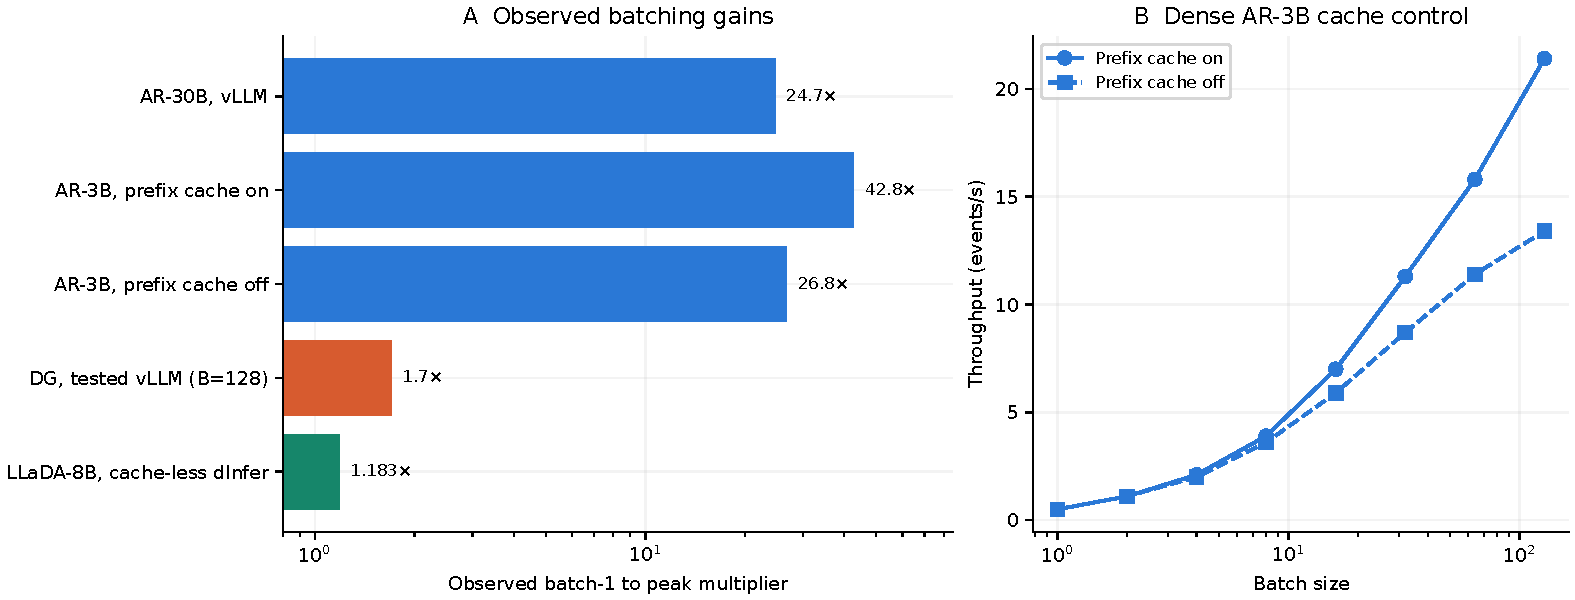
\includegraphics[width=\linewidth]{figures/fig6_batching.pdf}
\caption{Observed throughput multipliers for several model/runtime pairs.
The primary AR-30B result is approximately $25\times$. The cache-on/off
control uses dense AR-3B. Disabling cross-request
prefix caching lowers that model's multiplier from \cacheOnMult$\times$
to \cacheOffMult$\times$, so shared prefixes alone do not explain
its throughput gain. These controls do not identify a universal DG limit.}
\label{fig:batching}
\end{figure}

Sequential steps within one request chain cannot batch with each other,
but requests from independent chains can still overlap. Likewise,
interactivity and tenant isolation do not necessarily require a dedicated
batch-1 GPU. Deployment decisions should use measured arrival patterns,
scheduler behavior, and latency targets. Appendix~\ref{app:batching}
separates the cache observations from possible explanations.

\paragraph{Absolute and relative tails.}
In the repeated primary-pair measurements, AR-30B has CV
\arThirtyCV\% and max/median $1.75\times$, compared with
\dgThirtyCV\% and $3.07\times$ for DG. However, DG's absolute
p99 is \dgPninetyNine\,ms versus AR's \arPninetyNine\,ms.
A larger relative tail does not imply a slower absolute response or
a service-level agreement (SLA) violation. The relevant test is the specified latency percentile
under the intended arrival process. Sample maxima are not worst-case
bounds, and comparing maximum ratios across unequal sample sizes is
particularly fragile (Appendix~\ref{app:distributions}).

\paragraph{Prompt length and decoding settings.}
Longer prompts increase DG cost and can move the fitted crossover.
The input-slope comparison uses dense AR-3B and cannot be transferred
numerically to AR-30B. Canvas size and $K$ also change both cost and
quality. A joint sweep finds a better measured operating point than the
paper's reference setting: canvas 128, $K{=}8$ gives 368\,ms and
F1 0.864 versus 376\,ms and 0.853 at canvas 256, $K{=}8$.
These are point estimates on one sample, not a statistically established
improvement for all workloads (Appendix~\ref{app:input_canvas}).

\paragraph{Memory and co-residency.}
The nominal 52--60\,GB bf16 weight footprints of the primary pair
leave limited space for other large models on an 80\,GB GPU. Actual
capacity also depends on KV caches, activations, and runtime allocations.
A dense AR-1.5B has much smaller weights, but dividing GPU memory by
weight size cannot establish how many serving replicas fit or how their
throughput scales. We have not measured concurrent replicas, contention,
or isolation overhead, and make no linear co-residency speedup claim.

\paragraph{Cost accounting.}
At an assumed GPU rental rate $r$ dollars/hour, mean service time
$\bar t$ seconds/event, and busy fraction $u$, a simple single-instance
allocation is
\begin{equation}
 c_{\mathrm{event}}=\frac{r\bar t}{3600u}.
\end{equation}
This assumes the same GPU is rented throughout both busy and idle periods;
it excludes central processor, storage, networking, and retry costs. At fixed demand,
lower latency does not reduce the bill for an always-on GPU unless it
allows fewer provisioned resources or more useful work. A latency-based rental estimate therefore does not establish realized
annual savings. Batching economics should use measured throughput and
the quality requirement, rather than a serial latency ratio alone.

For a deadline-bound task, first establish which configurations return
acceptable records on time, then compare their costs. A configuration
that processes more records per second may still deliver each record too
late for that task. Conversely, the serial comparison does not show that
every AR configuration misses the target: scheduler, model, and decoding
choices require measurement at the intended load.

\subsection{Secondary-model chains and wider schemas}
\paragraph{Serial investigation chains.}
An investigation can require dependent steps: inspect an alert, retrieve
context, and choose a follow-up query. This makes serial model latency
relevant within a chain. The BGL chain harness compares DG with dense
AR-3B, at approximately 419 and 808\,ms per hop, respectively.
It does not directly measure an AR-30B chain or the retrieval and tool
latencies of a deployed investigation system.

\begin{figure}[ht!]
\centering
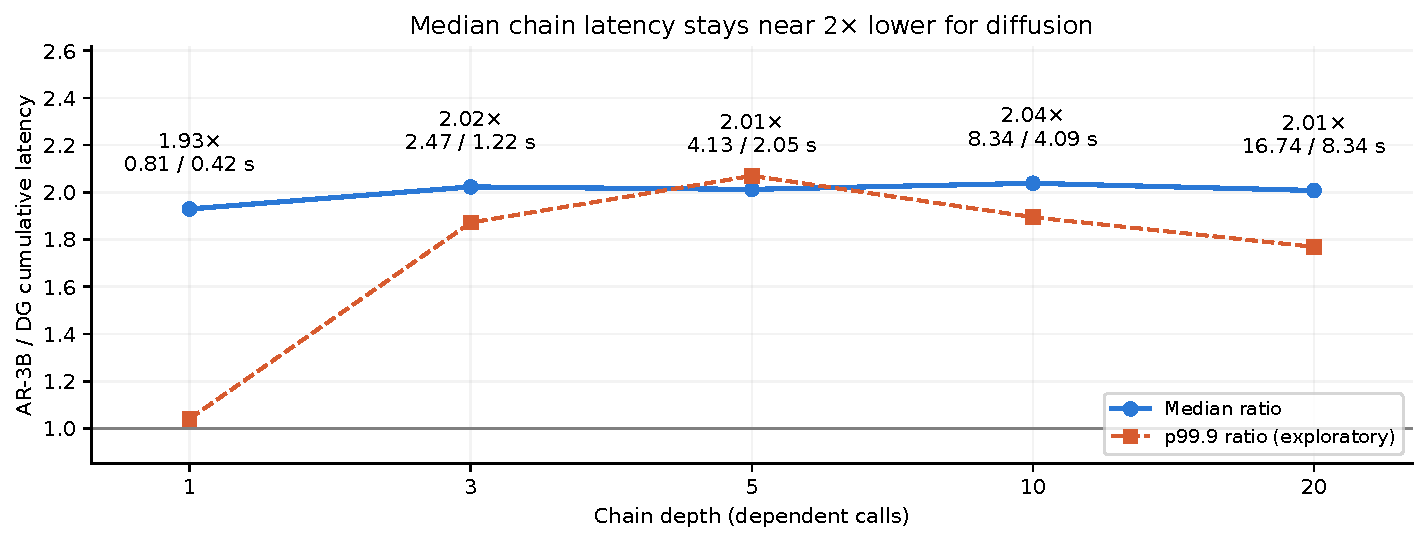
\includegraphics[width=\linewidth]{figures/fig10_usecase_chains.pdf}
\caption{AR/DG chain-latency ratios on BGL (DG versus dense AR-3B;
$n{=}100$ chains per depth, $K{=}8$). A ratio above one favors DG.
The median ratio stays near $2\times$; point labels give absolute cumulative
medians in seconds (AR / DG). The dashed p99.9 ratio is exploratory:
with 100 chains it reflects near-maximum observations, not a reliable
production tail target.}
\label{fig:chains}
\end{figure}

The latency gap accumulates when several dependent calls are required,
but neither the quality of a complete investigation nor independence of
hop latencies follows from this curve. The HumanEval correction-chain
artifact reports total-chain and first-round medians; those are not
per-round latency growth rates (Appendix~\ref{app:humaneval}).

\paragraph{Reducing effort before a deadline.}
DG exposes a denoising-effort control, $K$. In the BGL sweep, reducing
$K$ from 8 to 4 lowers quality from \kEightFone{} to \kFourFone{}
while yielding p99 \kFourPninetynine\,ms. This operating point
falls below a 400\,ms service-time budget in that sample. It does not
guarantee valid JSON, completion under arbitrary interruption, or a
400\,ms end-to-end deadline. Selecting a lower $K$ before generation
is different from safely preempting an unfinished canvas.

Under an output-length cap of 128 tokens, DG's schema validity falls to
\dgValidTwentyEight\%, compared with \arValidTwentyEight\% for
dense AR-3B. Thus lowering denoising effort and shortening the output
budget have different effects (Appendix~\ref{app:quality}). AR also
admits adaptive budgets, early stopping, retries, and routing policies;
we do not claim that adaptive computation is unique to diffusion.
Grammar-constrained AR remains an important unmeasured comparator.

\paragraph{Wide schemas.}
Across schemas with 12--100 fields, DG's measured latency advantage
against dense AR-3B ranges from approximately $1.8\times$ to
$3.0\times$. Both prompt and output lengths change, and the models
emit different token counts. This is a useful workload comparison,
but does not isolate a benefit from joint inter-field reasoning.
The consistency evaluator checks three fixed rules over four fields at
every width, so it cannot establish scaling with the number of
pairwise constraints.

\begin{figure}[ht!]
\centering
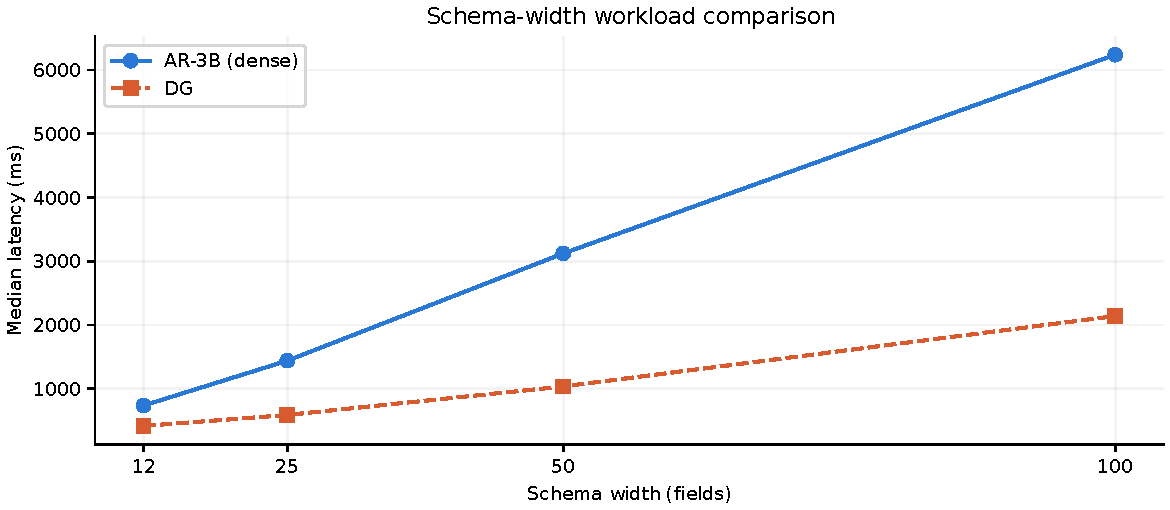
\includegraphics[width=0.85\linewidth]{figures/fig11_usecase_schema.pdf}
\caption{Latency versus schema width (BGL, $n{=}200$; dense AR-3B
baseline). DG's advantage rises from about $1.8\times$ to
$2.9$--$3.0\times$. Input length, output length, and canvas count
change together, preventing a causal attribution to schema width alone.}
\label{fig:schema}
\end{figure}

\paragraph{Adaptive effort: a measured negative result.}
A two-stage cascade first runs DG at $K{=}2$, checks structural-field
completeness, and reruns unresolved inputs at $K{=}8$. In the BGL
experiment ($n{=}200$), 29.5\% of records finish at the first stage
and 70.5\% escalate. F1 is 0.848 versus 0.853 for fixed $K{=}8$;
mean latency increases to 465\,ms from 376\,ms. The extra low-effort
pass costs more than it saves. Completeness is also only a proxy for
correctness. A lower escalation rate could improve this tradeoff, but
that benefit is not observed here.

\paragraph{Scope of application claims.}
The evidence concerns log extraction and exploratory code-generation
harnesses. We have not evaluated driving, trading, or deployed security
response, and do not infer suitability for those applications from
batch size or latency shape. Even in logs, the deployment choice depends
on quality, output validity, arrival rate, and the available AR baseline.
Appendix~\ref{app:refuted} reports the hypotheses that were contradicted
or left unsupported by the experiments.
